\documentclass[12pt]{article}
\usepackage[T1]{fontenc}
\usepackage{graphicx}
\graphicspath{{imagenes/}}

\begin{document}

\begin{flushleft}

\includegraphics[width=2.75cm]{unam.png}\hspace{8cm} 
\includegraphics[width=2.5cm]{fac.png}
\end{flushleft}

\begin{center}
\begin{Huge}
\texttt{UNAM}
\end{Huge}

\vspace{0.5cm}
\begin{LARGE}
\texttt{FACULTAD DE INGENIERIA}

\vspace{0.5cm}
\texttt{INGENIERIA EN COMPUTACION}

\vspace{0.5cm}
\texttt{PROGRAMACION ORIENTADA OBJETOS}

\vspace{0.5cm}
\texttt{MANUAL DE USUARIO PROYECTO HOTEL}

\vspace{1cm}
\end{LARGE}

\vspace{0.5cm}
\begin{LARGE}
\texttt{CARRILLO SANCHEZ RICARDO\\HERNANDEZ GOMEZ ALEJANDRO\\ZARAZUA RAMIREZ JOHAN AXEL}

\vspace{1cm}
\texttt{GRUPO: 04}

\vspace{1cm}
\texttt{PROFESOR: EDGAR TISTA GARCIA}
\end{LARGE}
\end{center}


\vspace{4cm}
\begin{flushleft}
\begin{Large}
\textbf{Manual de usuario del sistema de administración de hotel}
\end{Large}

\section{Requerimentos del sistema y proceso de instalación}

\textsf{Se deberá contar con un equipo con java JRE o JDK y una versión reciente del IDE Netbeans, sea para un  sistema operativo MAC OS, o Windows.\vspace{0.5cm} \\También es necesario contar con Mysql. Este programa o IDE debe de ser descargado de la página oficial de Mysql. }

\vspace{0.5cm}
\textsf{Una vez en su pagina oficia debemos ir a la sección Downloads  y aquí debemos de seleccionar la opcion MySQL Community (GPL) Downloads, que se encuentra en la parte de abajo, donde dependiendo de tu sistema y microarquitectura deberas escoger uno u otro instalador. Si cuentas con windows recomendamos que se descargue MySQL Installer for Windows. Este nos permitirá configurar algunos aspectos al instalar, es importante mencionar que al momento de instalar Mysql nos pedirá que ingresemos una contraseña para el usuario que nos da por defecto (root) y tendremos la opción de agregar un usuario, en este punto es esencial  crear un usuario con los campos:\\
Usuario : JohanZR\\
contraseña: 1602J\\
Host : All host\\
Role: DB Admin\\
Despues de esto continuas con la instalación hasta terminar.Esto si la computadora no cuneta con MySQl instalado, pero si la computadora ya cuenta con MySQL se deberá crear el usuario mediante comandos. Para crear el usuario desde comandos buscaremos en nuestra computadora "MySQL Command Line Client" y lo abriremos.}

\vspace{0.5cm}
\begin{center}
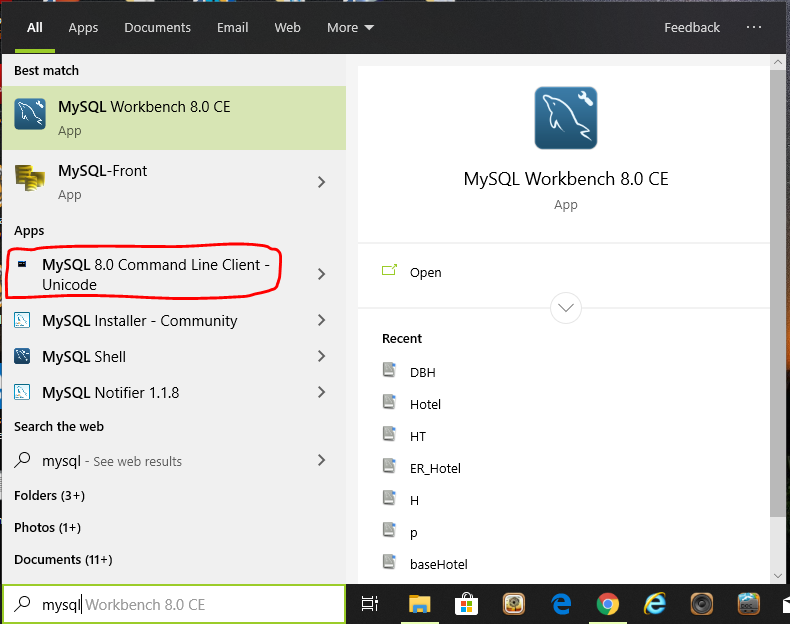
\includegraphics[width=10cm]{crearUsuario1.png}
\end{center}
\vspace{0.5cm}

\textsf{Una vez que abierto nos pedirá que introduzcamos la contraseña del usuario root, la ingresamos y posteriormente escribiremos el comando " create user JohanZR identified by '1602J'; ", este comando creara el usuario con su contraseña.}

\vspace{0.5cm}
\begin{center}
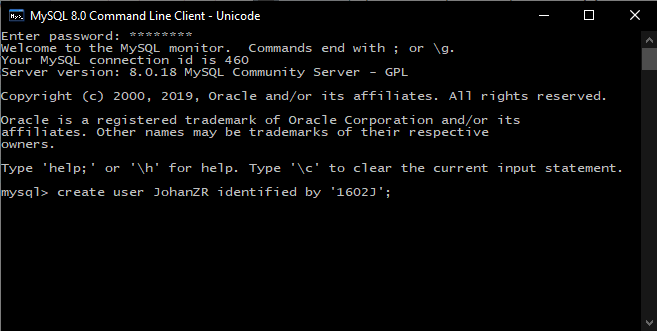
\includegraphics[width=10cm]{crearUsuario2.png}
\end{center}
\vspace{0.5cm}

\textsf{"Despues de esto se deberan modificar los privilegios del nuevo usuario para que tenga acceso a todas las bases de datos existentes, para esto debemos utilizar el comando " grant all privileges on *.* to 'JohanZR'; " y por ultimo utilizaremos el comando " flush privileges; " para refrescar.}

\vspace{0.5cm}
\begin{center}
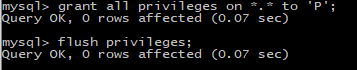
\includegraphics[width=10cm]{crearUsuario3.png}
\end{center}
\vspace{0.5cm}

\textsf{Es importante la creación de este usuario ya que la aplicación lo ocupara y sin este usuario creado no podemos garantizar el correcto funcionamiento de la misma sin realizar cambios la clase que se conectara con la base de datos.}


\vspace{0.5cm}
\textsf{Si no se sigue esta recomendación,se deberán realizar las modificaciones apropiadas en el código; específicamente en la clase Conexion del paquete logico del proyecto, donde se deberá modificar la variable user y password, Por ejemplo:  }

\vspace{0.5cm}
\begin{center}
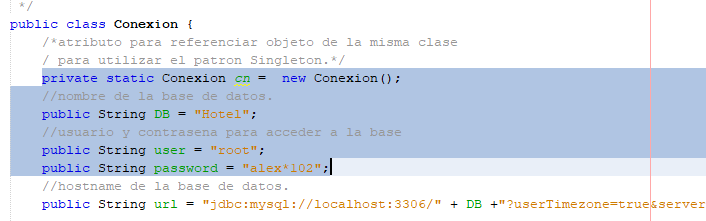
\includegraphics[width=10cm]{cambio.png}
\end{center}

\vspace{0.5cm}
\textsf{Una vez creado este el usuario JohanZr se debera abrir Workbench y crear una conexion con el nombre " Hotel ". La conexión se realiza  en el icono de la casita.}

\vspace{0.5cm}
\begin{center}
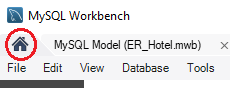
\includegraphics[width=10cm]{icono.png}
\end{center}

\vspace{0.5cm}
\textsf{En la parte de MySQL Connections tenemos que darle al símbolo mas y posteriormente nos abrirá otra ventana en la cual introduciremos los datos hostname =  localhost, puerto = 3306, ademas de los datos del usuario (JohanZR) y como nombre de la conexión la palabra Hotel}

\vspace{0.5cm}
\begin{center}
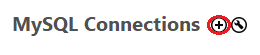
\includegraphics[width=7.5cm]{connection.png}
\end{center}

\vspace{0.5cm}
\begin{center}
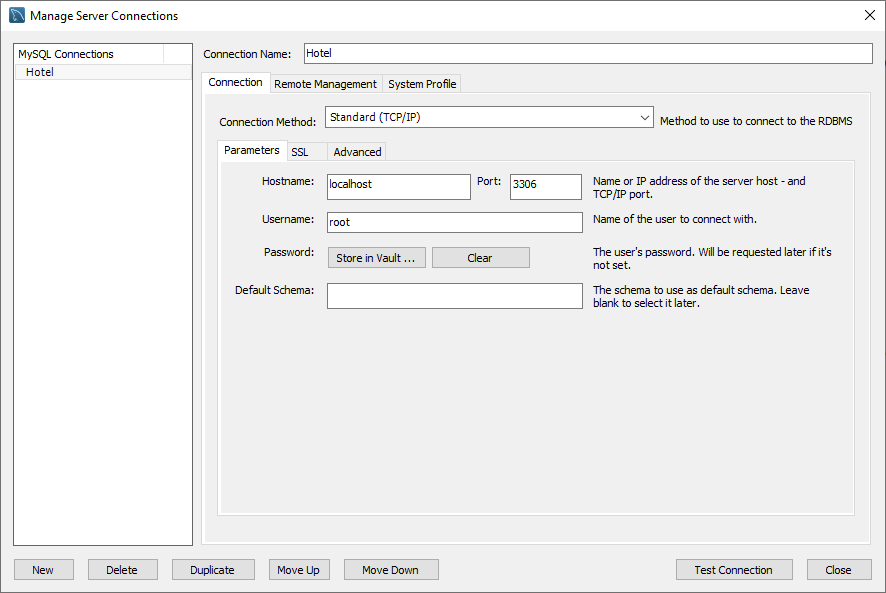
\includegraphics[width=10cm]{usuario.png}
\end{center}

\vspace{0.5cm}
\textsf{Probamos la conexión con Test Connection, si la conexión fue éxitosa abrirá una ventana emergente indicando dicho éxito y, si no, tenemos que verificar tanto el usuario como la contraseña sean correctos. Aparecerá la pantalla de incio de una conexion y nos dirigiremos a la parte de administration.}

\vspace{0.5cm}
\begin{center}
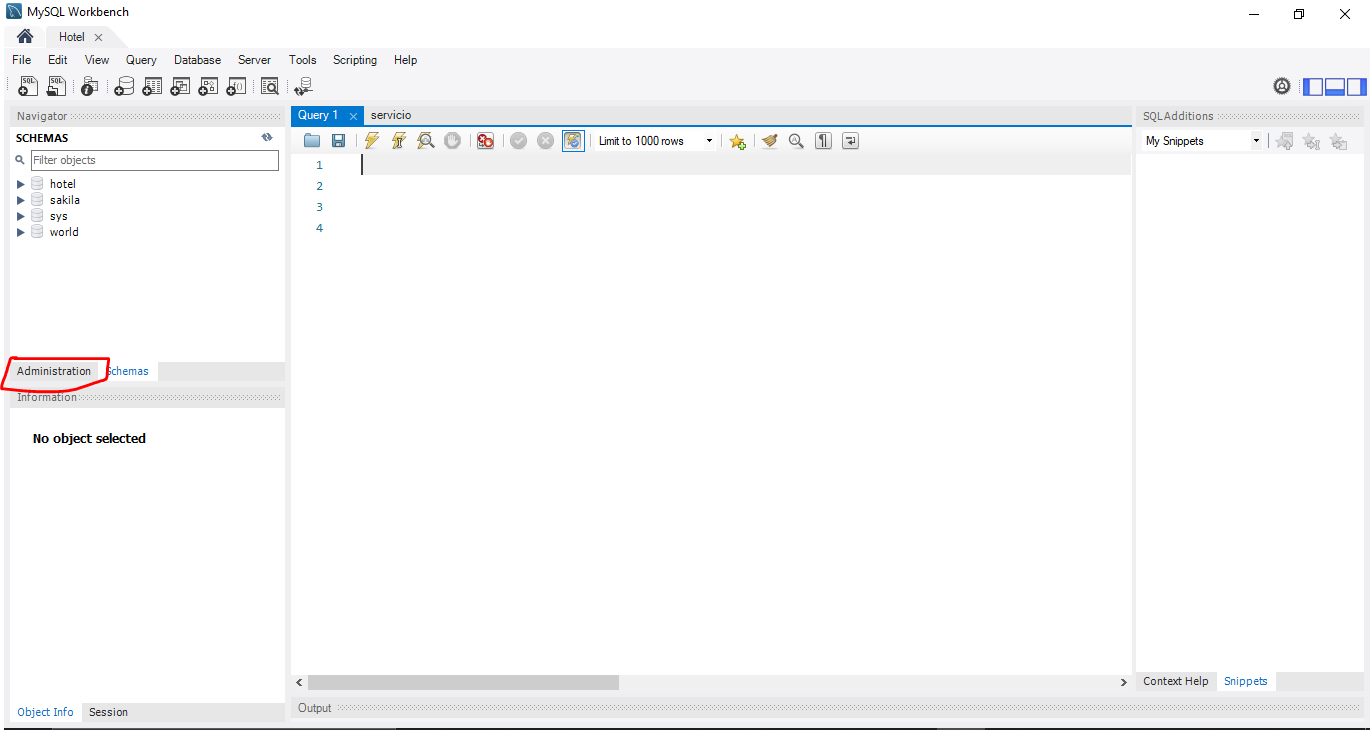
\includegraphics[width=10cm]{Johan1.png} 
\end{center}
\vspace{0.5cm}

\textsf{Una vez dentro de administration podremos ver distintas opciones, nos debemos dirigir a la opcion Data import/restore para poder crear la base de datos y que la aplicacion funcione de manera correcta.}

\vspace{0.5cm}
\begin{center}
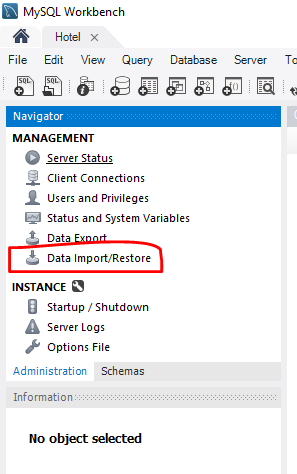
\includegraphics[width=4cm]{Johan2.png} 
\end{center}
\vspace{0.5cm}

\textsf{Esto nos generaara una venta y en ella deberemos seleccionar la opcion import from self contained file (1) aqui abriremos el archivo DBH(1) que se encuentra contenido en la carpeta del proyecto. Despues debemos apretar el boton new (2) y darle el nombre "hotel" al esquema (3). Por ultimo pasamos a la ventana import progress y en ella activaremos el botono start import (4). Con esto la base de datos quedara guardada y podremos comprobarlo en la ventana schemas.}

\vspace{0.5cm}
\begin{center}
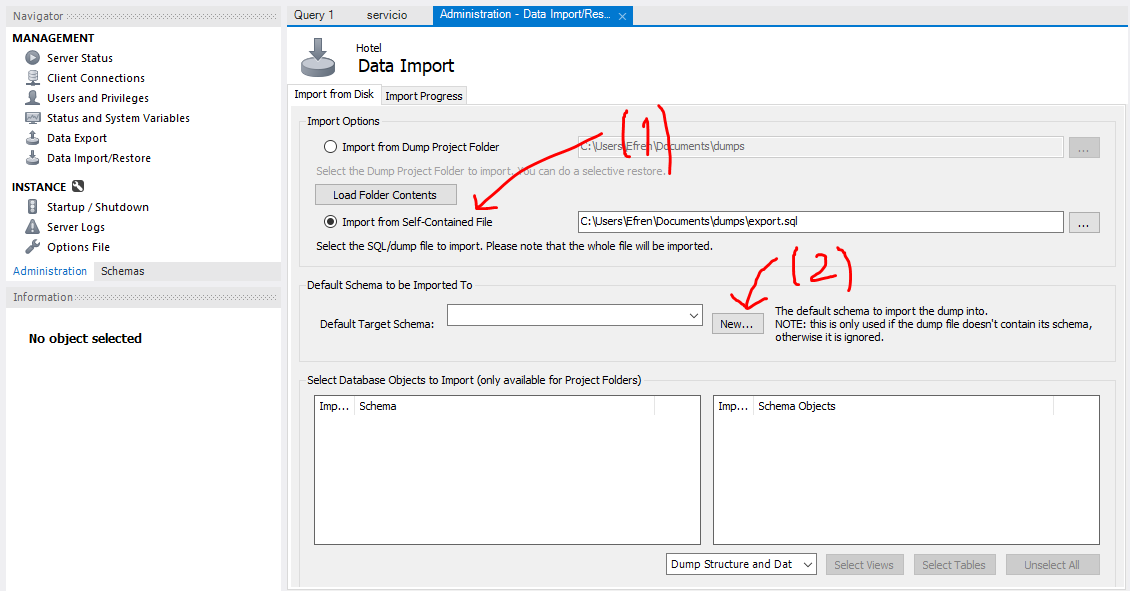
\includegraphics[width=10cm]{Johan3.png} 
\end{center}

\vspace{0.5cm}
\begin{center}
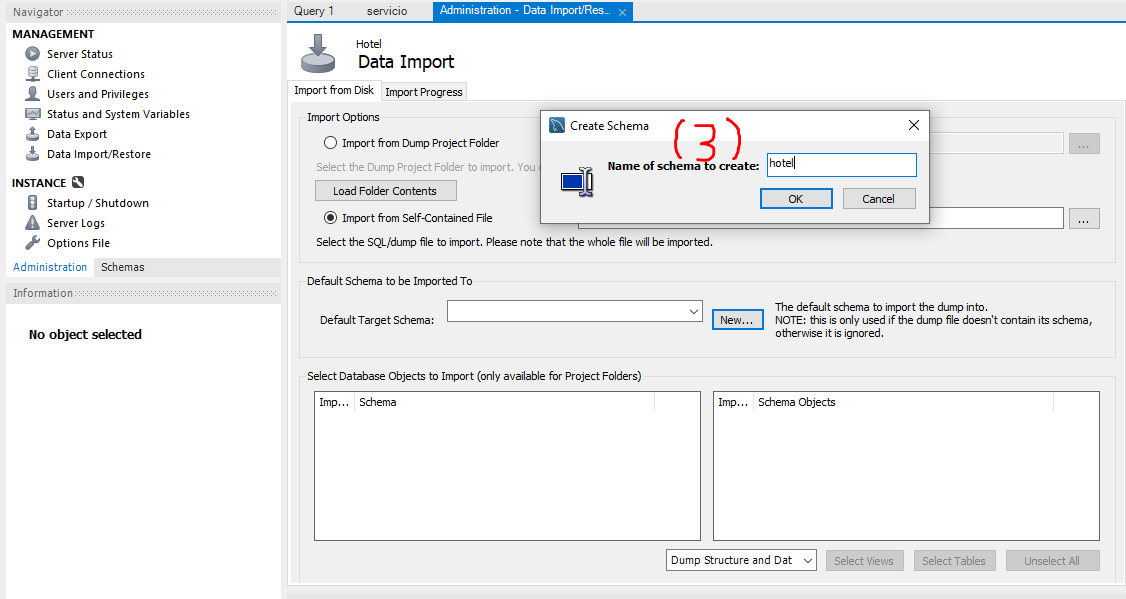
\includegraphics[width=10cm]{Johan4.png} 
\end{center}

\vspace{0.5cm}
\begin{center}
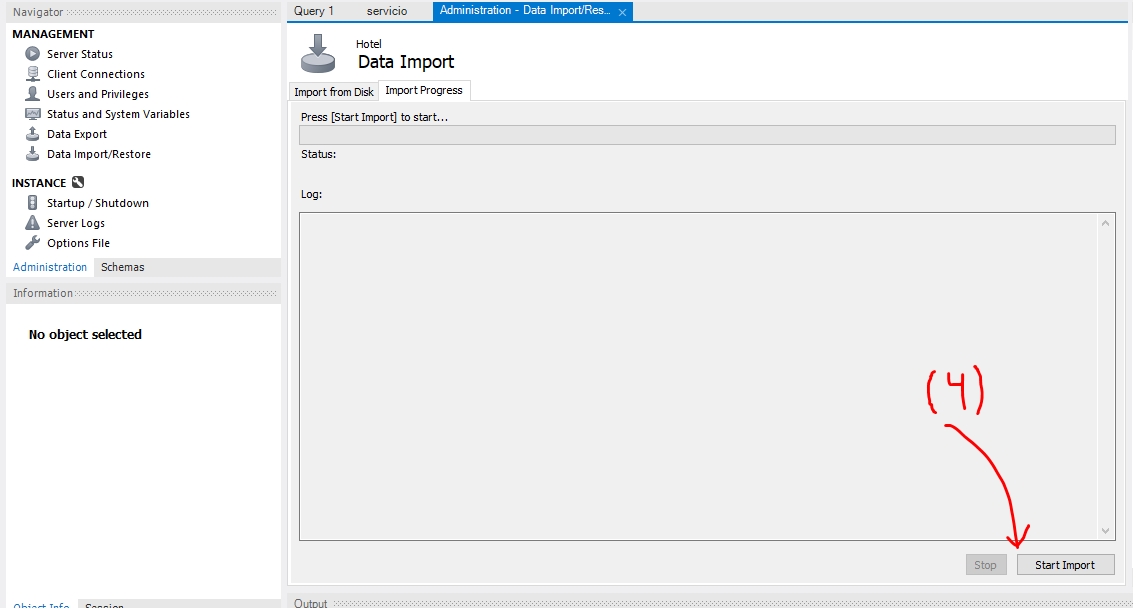
\includegraphics[width=10cm]{Johan5.png} 
\end{center}
\vspace{0.5cm}

\textsf{Una vez creada la base de datos podremos ejecutar el archivo .jar del proyecto el cual comenzara con el incio de sesion. Es importante mencionra que la base de datos ya cuenta con tres trabajadores registrados los cualos son:\\
user = johan  password = 1203a1602J@\\
user = ale  password = Spartan123\\
user = richi password = \\
Con los cuales podremos ingresar al sistema, sin embargo cada uno tiene puestos distintos por lo cual las acciones que puede realizar cada uno dentro del sistema son diferentes.}

\section{Inicio de sesión}
\textsf{Dentro del proceso de inicio de sesión se tiene que ingresar el usuario y contraseña de cliente o de trabajador que será proporcionado una vez que el cliente o el trabajador haya sido registrado. En caso de que el usuario olvide su contraseña podrá accionar el botón recuperar contraseña, esto le mostrara una venta en la cual se le pedirá que seleccione una pregunta de seguridad e ingrese la respuesta que registro al ser registrado en el sistema.  Una vez ingresado al sistema aparecerán las acciones que cada uno de los usuarios pueden realizar\vspace{0.5cm} \\Los trabajadores tendrán diferentes acciones disponibles segán el tipo de trabajador que sean. Las acciones que pueden realizar son las siguientes: }

\vspace{0.5cm} 

\begin{itemize}
\item{\textbf{Registrar habitaciones } disponible para (Director, Gerente)}
\item{\textbf{Registrar servicios} disponible para (Director, Gerente)}
\item{\textbf{Registrar reservaciones }disponible para (Director, Gerente, Subgerente, Recepcionista)}
\item{\textbf{Registrar clientes } disponible para (Director, Gerente, Subgerente, Recepcionista)}
\item{\textbf{Registrar trabajadores} disponible para (Director, Gerente)}
\item{\textbf{Registrar pagos } disponible para (Director, Gerente, Subgerente, Recepcionista)}
\item{\textbf{Registrar compras } disponible para (Director, Gerente, Subgerente, Recepcionista)}
\item{\textbf{Consulta  de algún campo} disponible para (TODOS)}
\end{itemize}

\section{Registrar habitaciones}
\textsf{Para poder registrar habitaciones será necesario ser un director o gerente. El proceso inicial será seleccionar la opción de Registrar habitaciones y se proseguirá a llenar la ventana emergente para el registro, en la cual nos concentraremos principalmente en la parte izquierda de la ventana, tal y como se muestra a continuación: }
\vspace{0.5cm}
\begin{center}
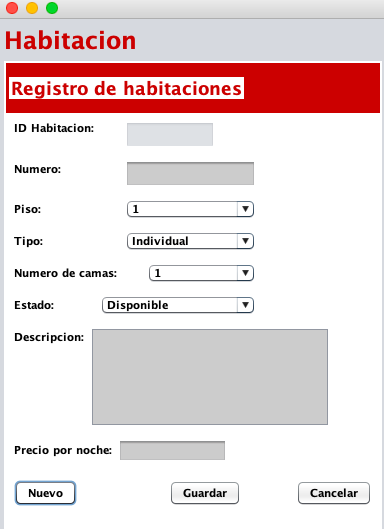
\includegraphics[width=7.75cm]{1.png}
\end{center}
\vspace{0.5cm}
\textsf{Las opciones se encontraran bloqueadas hasta que el usuario oprima el botón "Nuevo", el cual habilitara los campos necesarios para realizar el registro\vspace{0.5cm} \\Será necesario proporcionar todos los campos para completar un registro, de otra forma aparecerá una ventana emergente como la siguiente: }
\vspace{0.5cm}
\begin{center}
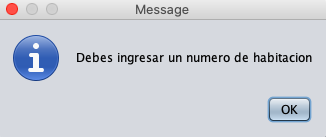
\includegraphics[width=7.75cm]{2.png}
\end{center}
\textsf{Donde el error cometido en este caso habría sido no colocar el campo número de habitación\\}
\vspace{0.5cm}
\textbf{Advertecia: El sistema acepta números de habitación repetidos; en caso de cometer un error de este tipo o algún otro similar vease la opción eliminar o editar en esta misma sección.\\}
\vspace{0.5cm}
\textsf{Una vez que se haya terminado el llenado de los campos requeridos se tiene guardar el registro con el su botón correspondiente. Teniendo el registro guardado, se confirmara con la siguiente ventana emergente: }
\vspace{0.5cm}
\begin{center}
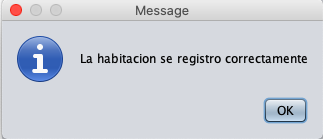
\includegraphics[width=7.75cm]{4.png}
\end{center}
\textsf{A su vez en la ventana derecha, se nos mostrara el registro que realizamos.}
\vspace{0.5cm}
\begin{center}
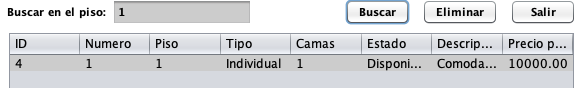
\includegraphics[width=12.75cm]{3.png}
\end{center}
\textsf{El complemento de la ventana que se encuentra a la derecha, servirá para que el usuario pueda visualizar los registros que este haya creado, buscar algún registro o eliminar algún registro erróneo o no deseado.\vspace{0.5cm} \\La sección buscar en el piso, nos permitirá hacer un filtro de los registros realizados por piso ingresado. El hotel cuenta con 12 pisos y en caso de escribir un piso no valido, simplemente no se mostrarán registros.\vspace{0.5cm} \\Para eliminar un registro será necesario seleccionar el registro a eliminar y para hacerlo bastara con hacer click en el, por ultimo se debe presionar el botón eliminar.}
\vspace{0.5cm}
\begin{center}
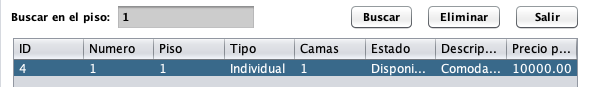
\includegraphics[width=12.75cm]{5.png}
\end{center}
\textsf{Para editar algún campo de un registro se debe precionar en la opcion que se desea modificar, y se habilitará la opción para poder editar el campo que desamos y una vez modificado se deberá confimar pulsando enter. }
\vspace{0.5cm}
\begin{center}
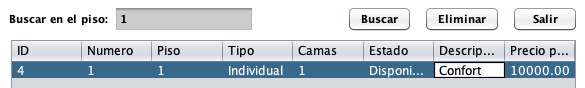
\includegraphics[width=12.75cm]{6.png}
\end{center}
\textbf{Advertecia: Esta opción se encuentra en mantenimiento, es posible que no se logren editar los registros exitosamente.\\}



\section{Registro de servicios}
\textsf{Para poder registrar servicios será necesario ser un director o gerente. El proceso inicial será seleccionar la opción de Registrar servicios y se proseguirá a llenar la ventana emergente para el registro, en la cual nos concentraremos principalmente en la parte izquierda de la ventana, tal y como se muestra a continuación: }
\vspace{0.5cm}
\begin{center}
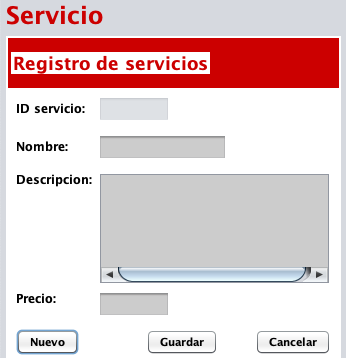
\includegraphics[width=7.75cm]{7.png}
\end{center}
\vspace{0.5cm}
\textsf{Las opciones se encontraran bloqueadas hasta que el usuario oprima el botón "Nuevo", el cual habilitara los campos necesarios para realizar el registro\vspace{0.5cm} \\Será necesario proporcionar todos los campos para completar el registro, de otra forma aparecerá una ventana emergente como la siguiente: }
\vspace{0.5cm}
\begin{center}
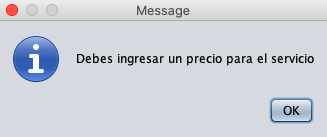
\includegraphics[width=7.75cm]{8.png}
\end{center}
\textsf{Donde el error cometido en este caso habría sido no colocar el campo precio del precio del servicio\\}
\vspace{0.5cm}
\textsf{Una vez que se haya terminado el llenado de los campos requeridos se tiene guardar el registro con el su botón correspondiente. Teniendo el registro guardado, se confirmara con la siguiente ventana emergente: }
\vspace{0.5cm}
\begin{center}
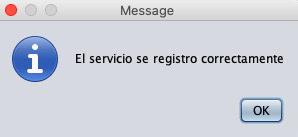
\includegraphics[width=7.75cm]{9.png}
\end{center}
\textsf{El complemento de la ventana que se encuentra a la derecha, servirá para que el usuario pueda visualizar los registros que este haya creado, editar algún registro o eliminar algún registro erróneo o no deseado.\vspace{0.5cm} \\Para editar un registro será necesario seleccionar el registro a editar y para hacerlo bastara con hacer click en el y en la ventana derecha se nos habilitaran  los campos donde previamente llenamos la información, que será donde se tendrá que escribir la nueva información que desearemos editar. Por ultimo deberemos presionar nuevamente el botón "Editar" y se nos confirmara que hemos modificado el registro con la siguiente ventana emergente: }
\vspace{0.5cm}
\begin{center}
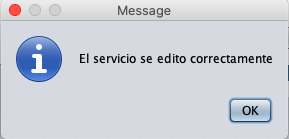
\includegraphics[width=7.75cm]{10.png}
\end{center}
\textsf{A su vez seremos capaces de observar el campo modificado a la derecha nuestra tabla de registros creados: }
\vspace{0.5cm}
\begin{center}
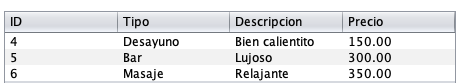
\includegraphics[width=12.75cm]{11.png}
\textsf{\\Registro sin Editar}
\end{center}
\vspace{0.5cm}
\begin{center}
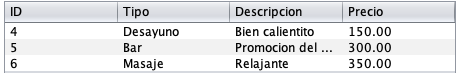
\includegraphics[width=12.75cm]{12.png}
\textsf{\\Registro 5 editado en el campo Descripcion}
\end{center}
\textsf{Para eliminar un registro será necesario seleccionar el registro a  y haciendo click en el, una vez seleccionado se deberá presionar el botón de eliminar, Esto nos arrojara una ventana emergente de confirmación para eliminar el registro correspondiente, de ser aceptada eliminara el registro}
\vspace{0.5cm}
\begin{center}
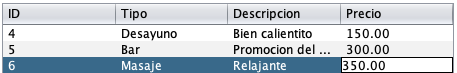
\includegraphics[width=12.75cm]{13.png}
\textsf{\\Seleccion del registro a eliminar}
\end{center}
\vspace{0.5cm}
\begin{center}
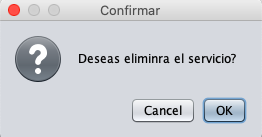
\includegraphics[width=7.75cm]{14.png}
\textsf{\\Ventana emergente para la confirmación del usuario}
\end{center}
\vspace{0.5cm}
\begin{center}
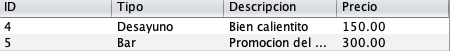
\includegraphics[width=12.75cm]{15.png}
\textsf{\\Lista después de eliminar el registro}
\end{center}




\section{Registro clientes}
\textsf{Para poder registrar clientes será necesario ser un director, gerente, subgerente o recepcionistas. El proceso inicial será seleccionar la opción de clientes de la parte Reservaciones y se proseguirá a llenar la ventana emergente para el registro, en la cual nos concentraremos principalmente en la parte izquierda de la ventana, tal y como se muestra a continuación: }
\vspace{0.5cm}
\begin{center}
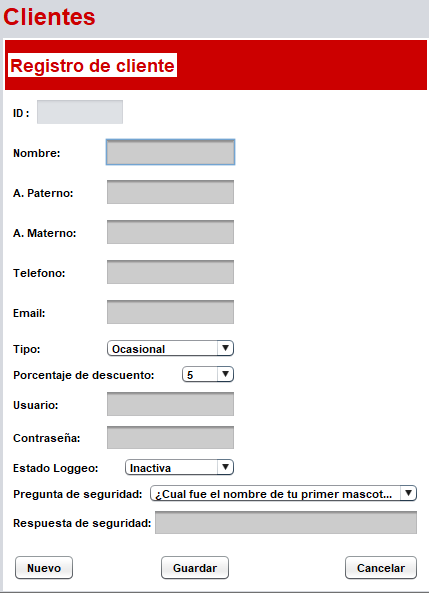
\includegraphics[width=7.75cm]{cliente.png}
\end{center}
\vspace{0.5cm}
\textsf{Las opciones se encontraran bloqueadas hasta que el usuario oprima el botón "Nuevo", el cual habilitara los campos necesarios para realizar el registro.}

\vspace{0.5cm} 
\textsf{Será necesario proporcionar todos los campos para completar el registro, de otra forma aparecerá una ventana emergente como la siguiente:}

\vspace{0.5cm}
\begin{center}
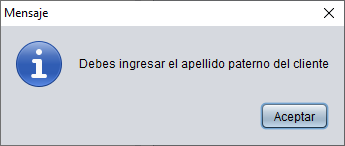
\includegraphics[width=7.75cm]{e_cliente.png}
\end{center}

\vspace{0.5cm}
\textbf{Advertecia: La contraseña debe contener como mínimo 8 caracteres el número telefónico al menos 10 dígitos.}

\vspace{0.5cm}
\begin{center}
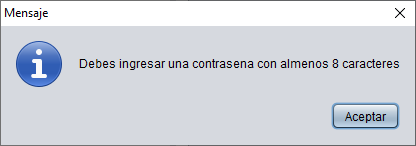
\includegraphics[width=7.75cm]{contra.png}
\end{center}
\begin{center}
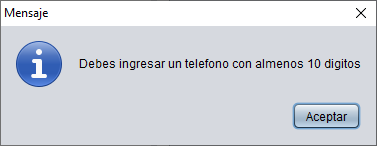
\includegraphics[width=7.75cm]{telefono.png}
\end{center}

\vspace{0.5cm}
\textsf{Una vez que se haya terminado el llenado de los campos requeridos se tiene guardar el registro con el su botón correspondiente. Teniendo el registro guardado, se confirmara con la siguiente ventana emergente: }
\vspace{0.5cm}
\begin{center}
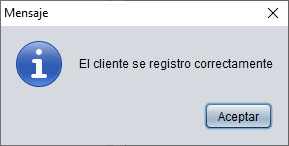
\includegraphics[width=7.75cm]{r_cliente.png}
\end{center}

\vspace{0.5cm}
\textsf{El complemento de la ventana que se encuentra a la derecha, servirá para que el usuario pueda visualizar los registros que este haya creado, editar algún registro o eliminar algún registro erróneo o no deseado.}
\vspace{0.5cm}
\begin{center}
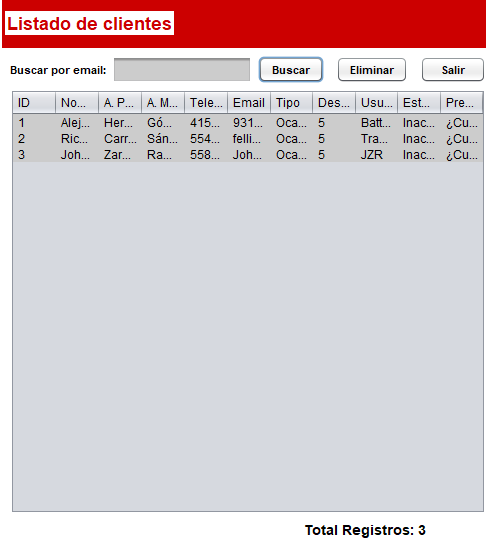
\includegraphics[width=7.75cm]{re_cliente.png}
\end{center}

\vspace{0.5cm}
\textsf{Las acciones de editar y eliminar son parecidas a las de registro de servicios. El único cambio en el apartado del listado es que la búsqueda es a través del correo electrónico.}



\section{Registro reservación}
\textsf{Para poder registrar clientes será necesario ser un director, gerente, subgerente o recepcionista. El proceso inicial será seleccionar la única opción de Configuración.}

\vspace{0.5cm}
\textsf{Este proceso va de la mano con otros sub procesos de registro, ya que para ello, se tuvo que haber registrado previamente a un cliente y una habitación, almacenandolos en la base de datos.}

\vspace{0.5cm}
\textsf{La acción para crear un nuevo registro es similar al de los registros pasados, todo se encuentra bloqueado hasta que que seleccionemos el botón nuevo}
\vspace{0.5cm}
\begin{center}
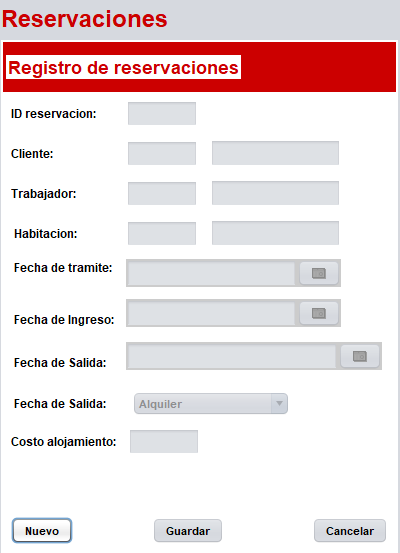
\includegraphics[width=7.75cm]{reservacion.png}
\end{center}

\vspace{0.5cm}
\textsf{Al crear un nuevo registro nos solicita una habitación y un cliente a relacionar con la reservación. De la base de datos podemos obtenerlos de sus respectivas tablas. Cada uno de ellos se puede buscar por los campos previamente definidos}
\vspace{0.5cm}
\begin{center}
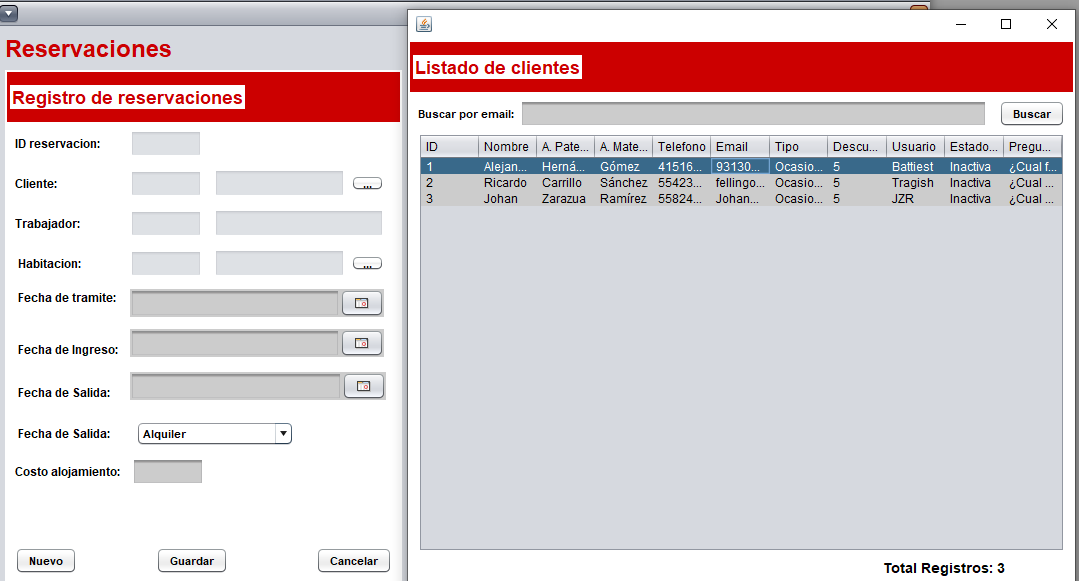
\includegraphics[width=7.75cm]{reserva_cliente.png}
\end{center}
\begin{center}
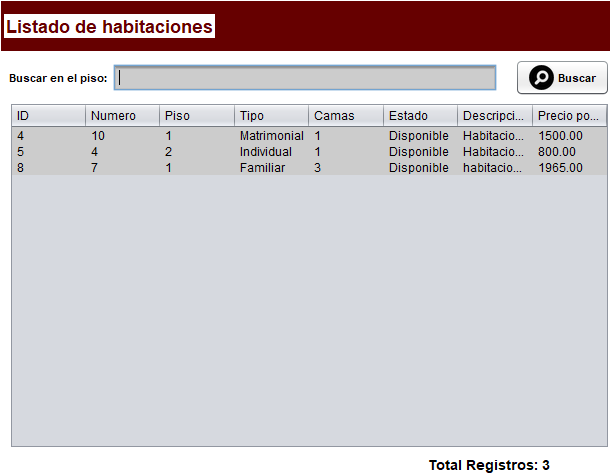
\includegraphics[width=7.75cm]{lis_habitacion.png}
\end{center}

\vspace{0.5cm}
\textsf{Para seleccionar la fecha únicamente tenemos que dar click en el cuadrito del calendario, dentro podemos elegir el mes, año y día. Día es lo último que debemos seleccionar, ya que al indicarlo devuelve la fecha elegida.}
\vspace{0.5cm}
\begin{center}
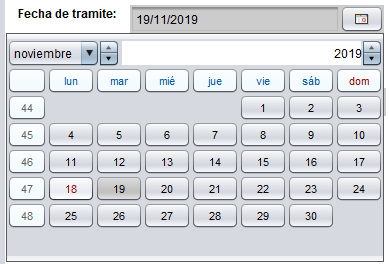
\includegraphics[width=7.75cm]{fecha.png}
\end{center}

\vspace{0.5cm}
\textsf{Como venimos repitiendo, todos los campos deben de estar llenos}

\vspace{0.5cm}
\textsf{El complemento de la ventana que se encuentra a la derecha, servirá para que el usuario pueda visualizar los registros que este haya creado, editar algún registro o eliminar algún registro erróneo o no deseado.}
\vspace{0.5cm}
\begin{center}
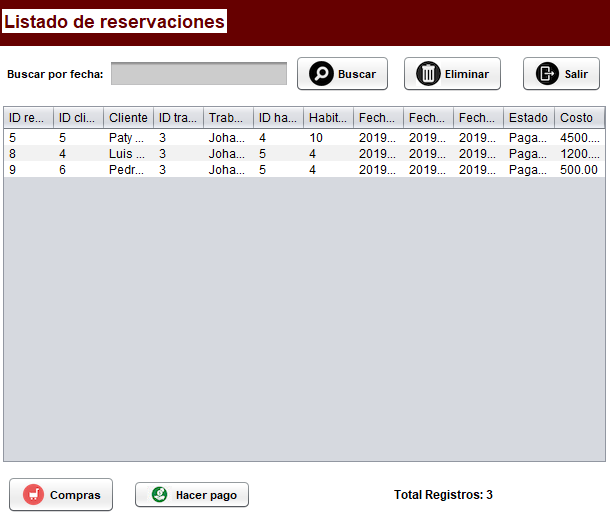
\includegraphics[width=7.75cm]{reset.png}
\end{center}

\vspace{0.5cm}
\textsf{Las acciones de editar y eliminar son parecidas a los registros. El único cambio en el apartado del listado es que la búsqueda es a través de la feccha de trámite.}



\section{Registro trabajadores}
\textsf{Para poder registrar clientes será necesario ser un director o gerente. El proceso inicial será seleccionar la única opción de Configuración.}

\vspace{0.5cm}
\textsf{Nuevamente los campos aparecerán bloqueados hasta que vayamos a crear un nuevo trabajador. El proceso es exactamente igual al de cliente; todos los campos deben de llenarse, las advertencias son las mismas y la búsqueda en la tabla de listados es igual por correo electrónico. Obviamente los campos varían en función al trabajador.}
\vspace{0.5cm}
\begin{center}
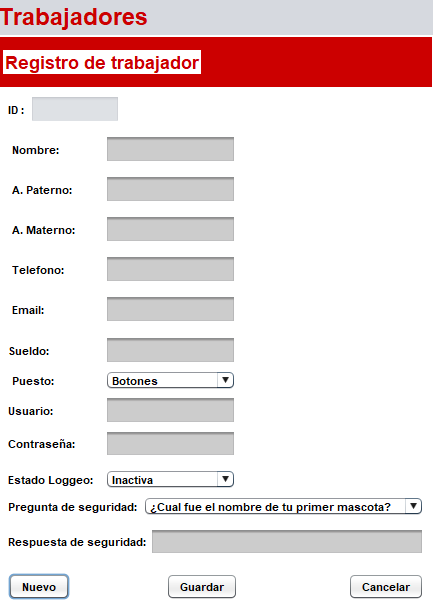
\includegraphics[width=7.75cm]{trabajador.png}
\end{center}

\vspace{0.5cm}
\begin{center}
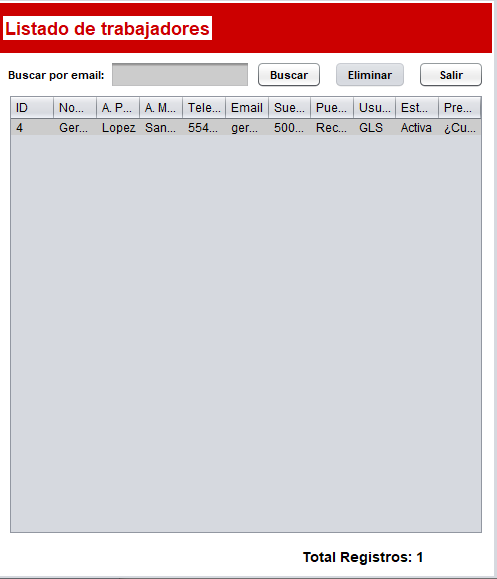
\includegraphics[width=7.75cm]{lis_trabajador.png}
\end{center}









\section{Registro pagos}
\textsf{Para poder registrar clientes será necesario ser un director, gerente, subgerente o recepcionista. Esta interfaz surge gracias al registro de reservaciones, para poder abrirla es necesario seleccionar en la tabla de listados una reservación y posteriormente dar click en el botón "Hacer pago"}

\vspace{0.5cm}
\begin{center}
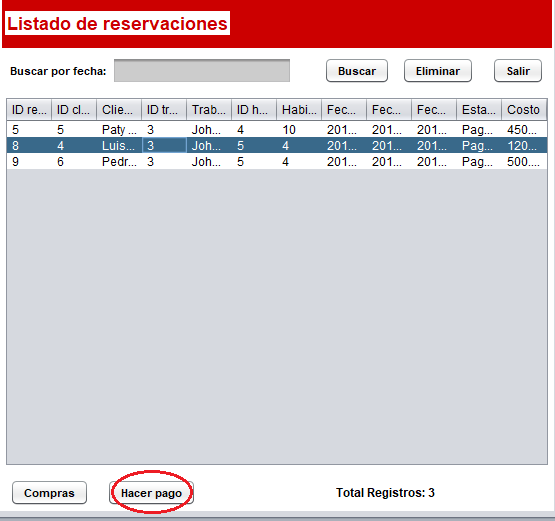
\includegraphics[width=7.75cm]{hacerpago.png}
\end{center}

\vspace{0.5cm}
\textsf{Nuevamente los campos aparecerán bloqueados hasta que vayamos a crear un nuevo pago. El proceso es exactamente igual a los anteriores; todos los campos deben de llenarse, las advertencias son las mismas y tiene sus campos característicos.}

\vspace{0.5cm}
\begin{center}
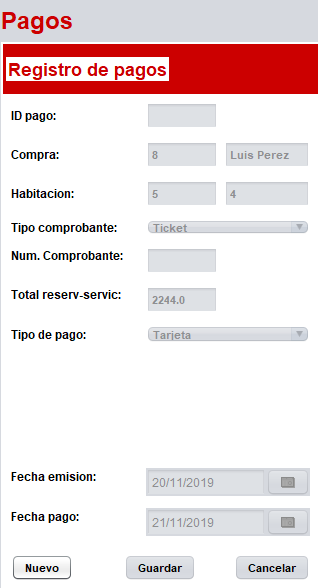
\includegraphics[width=7.75cm]{re_pagos.png}
\end{center}

\vspace{0.5cm}
\textsf{En el lado derecho aparecen dos tablas: listado de servicios y listado de pagos; ambas tablas no conservan el método de búsqueda, ya que en esta ocasión es tratado como una consulta de la propia interfaz. En el apartado de servicios únicamente vemos los servicios correspondientes a la reservación, el precio de la reservación, el precio total de los servicios y  el total de compras}

\vspace{0.5cm}
\begin{center}
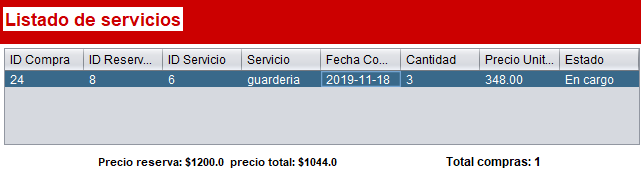
\includegraphics[width=7.75cm]{serv.png}
\end{center}

\vspace{0.5cm}
\textsf{Por otra parte, listado de pagos permite eliminar algún registro de pago o incluso editar sobre el seleccionado. Estos procesos también son similares a los anteriores de editar y eliminar.}

\vspace{0.5cm}
\begin{center}
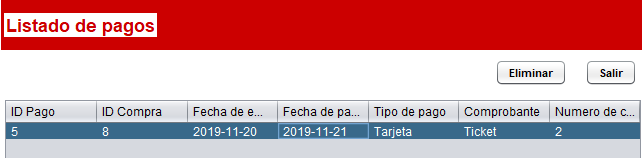
\includegraphics[width=7.75cm]{pagos.png}
\end{center}
\vspace{0.5cm}

\textsf{Es importa mencionar que al guardar un pago se crea un archivo pdf como comprobante de pago.}

\vspace{0.5cm}
\textsf{En la misma sección(menú de la interfaz principal), en la opción de pagos es posible consultar cada uno de ellos al igual que eliminar dependiendo de la decisión del usuario; es una tabla que se viene manejando a lo largo de la aplicación con los botones de buscar, eliminar y salir. La búsqueda es a través del id de pagos, es el listado total de pagos de todas las reservaciones creadas. El punto general de esta agrupación de datos.}

\vspace{0.5cm}
\begin{center}
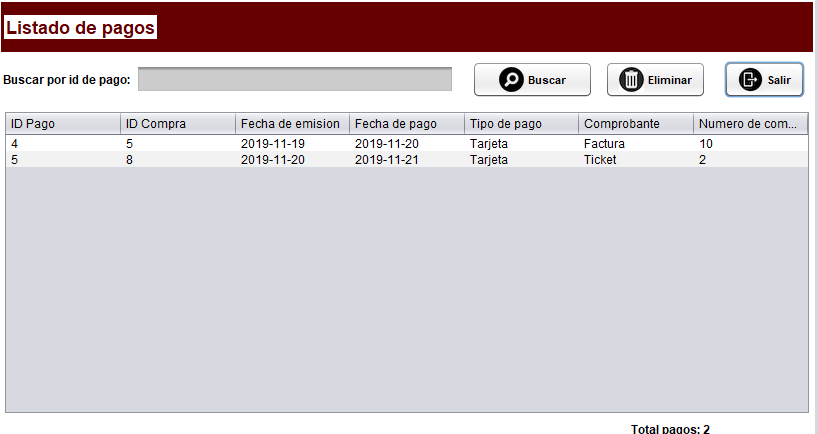
\includegraphics[width=7.75cm]{pagg.png}
\end{center}




\section{Registro compras}
\textsf{Para poder registrar clientes será necesario ser un director, gerente, subgerente o recepcionista. El proceso para abrir la interfaz es idéntico al de registro pagos, sólo tenemos que seleccionar una reservación y dar click en compras}

\vspace{0.5cm}
\begin{center}
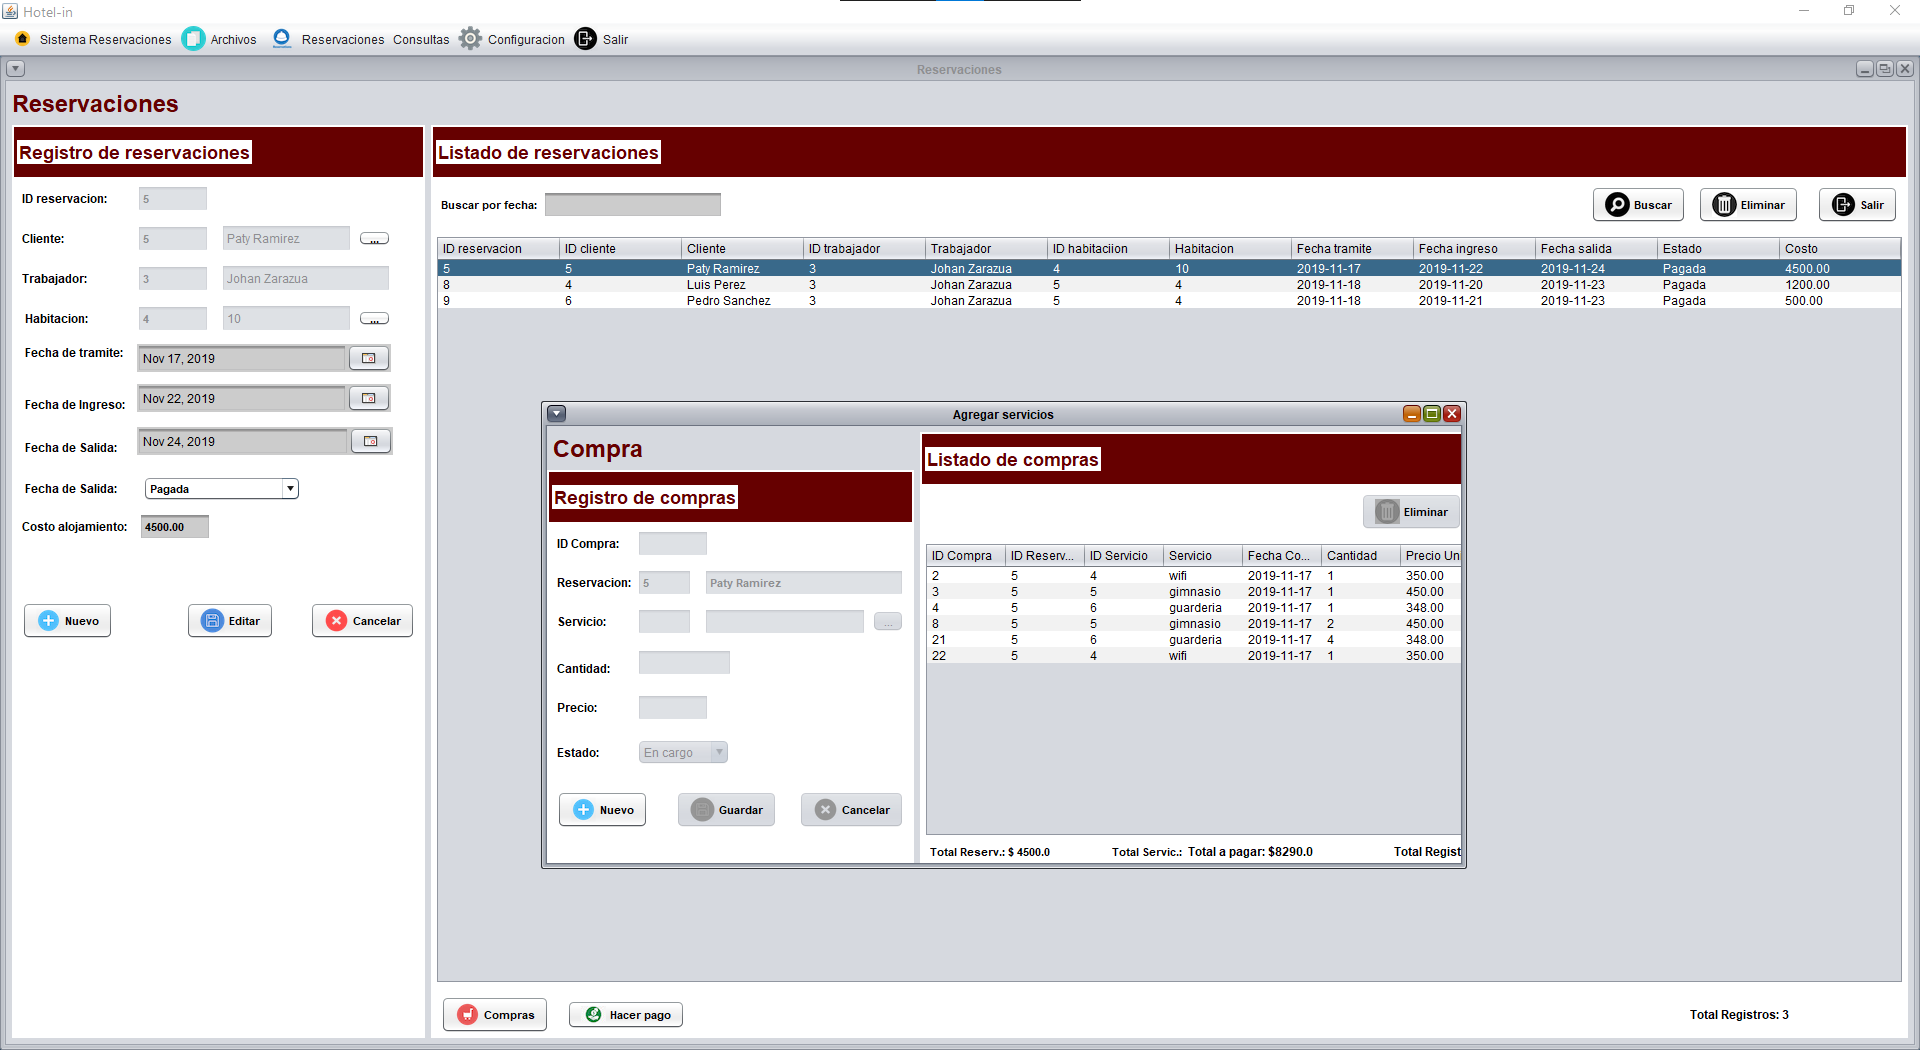
\includegraphics[width=7.75cm]{compras.png}
\end{center}

\vspace{0.5cm}
\textsf{Tras abrir la nueva ventana se hace costumbre los pasos para crear el registro de cualquier tipo de dato, o en esta ocasión, de categoría. Para realizar el registro de manera adecuada tiene que haber sido registrado previamente al menos un servicio, debido a que es un elemento fundamental de la compra.}

\vspace{0.5cm}
\begin{center}
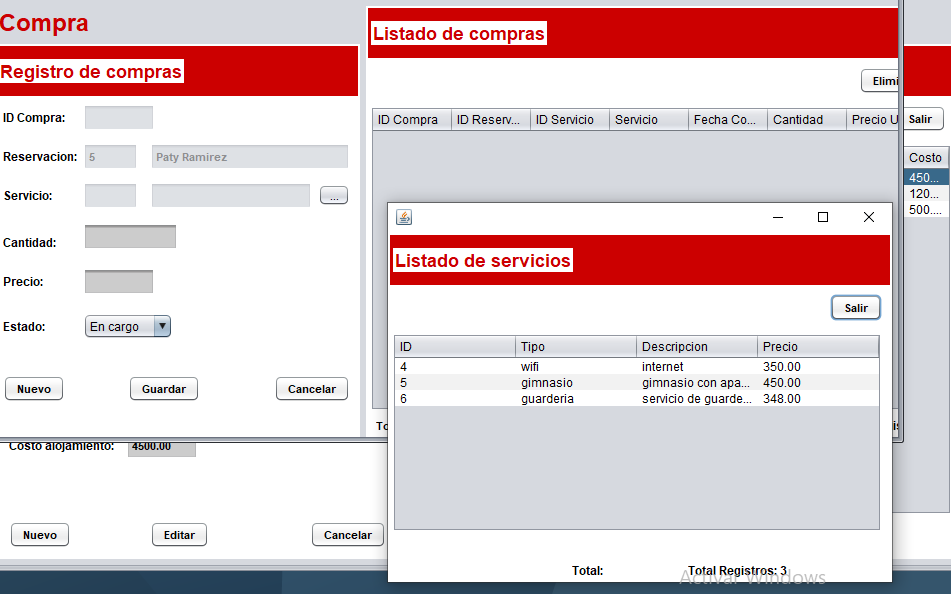
\includegraphics[width=7.75cm]{ec.png}
\end{center}

\vspace{0.5cm}
\textsf{La base de datos de compras aparece reflejada en el lado derecho, dándonos las opciones de eliminar o editar la compra. Los elementos en compras no son más que un complemento de pagos, uno puede tener, como se vió reflejado en el apartado de pagos, servicios que contribuyen al uamento del precio total o puede no tener alguna compra, con la reservación es más que suficiente para crear el pago}

\vspace{0.5cm}
\begin{center}
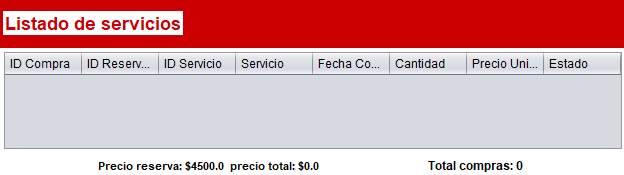
\includegraphics[width=7.75cm]{nocompra.png}
\end{center}

\section{Consulta de comprobantes de pago}
\textsf{Por ultimo se creo un menú Consultas en el cual existe un item llamado "Reservaciones clientes" este item se pude abrir dando click o presionando las teclas Ctrl+Shift+R. Al ingresar aquí podremos ver una pantalla en la cual nos pedirá que seleccionemos un tipo de comprobante y ingresemos el id de la reservacion, después se debe dar en el botón buscar y esto nos mostrar un ventana con todas  las direcciones de nuestra computadora, esta nos servirá para abrir el archivo pdf, al estar en esta ventana debemos dirigirnos a la localidad donde se encuentre la carpeta de la aplicación, entrar en esta carpeta posteriormente entrar a la carpeta "Hotel" que es en la que se encuentra el programa(.jar), una vez dentro de Hotel debemos ir a la carpeta src, después a hotel y por ultimo comprobantes, en esta ultima se encuentran todos los comprobantes de pago generados y se deberá seleccionar el archivo que tenga por nombre el id de la reservacion mas el tipo de comprobante que es ("f" si es Factura y "t" si es ticket) esto nos abrirá directamente el comprobante y podremos hacer múltiples acciones con el como imprimir, enviar,etc.}

\begin{center}
\includegraphics[width=7.75cm]{comprobante1.png}
\includegraphics[width=7.75cm]{comprobante2.png}
\includegraphics[width=7.75cm]{comprobante3.png}
\includegraphics[width=7.75cm]{comprobante4.png}
\end{center}



\end{flushleft}
\end{document}
